\subsubsection*{Project 1: Investigate structural modifications of irradiated silica for nuclear materials}\label{lang}

The first project would be the study of the local structure changes in amorphous silica ($ \textrm{SiO}_2 $) before and after irradiation of high energy
(tens of MeV or more) heavy ion bombardment, or swift heavy ions (SHIs). At these high energies, electronic stopping dominates over nuclear stopping, implying the SHI interacts with the electronic structure of the irradiated target material \cite{Klaumunzer2004136, Krasheninnikov2010, Weber2015}. The SHI path deposits energy to the electronic structure which then dissipates the energy to the nuclei of the atoms via kinetic energy, causing a local heat spike in the material radially outward perpendicular to the SHI pathway. In Figure \ref{shi_track}, we show models of quartz (crystalline silica) before and after a SHI bombardment event, looking directly down the SHI pathway through the material. In (a) and (b), we simply color the atoms by type where silicon atoms are \color{Dandelion} yellow \color{black} and the oxygen atoms are \color{BrickRed} red \color{black}. In (c) and (d), we color the atoms by their velocity, where the velocity scale increases going from \color{BrickRed} red \color{black} $\to$ \color{Dandelion} yellow \color{black} $\to$ \color{black} white. The black circles in (b) and (d) show the amorphized region of the quartz due to the large deposition of kinetic energy in the material.

\begin{wrapfigure}{r}{0.48\textwidth}
  \begin{center}
    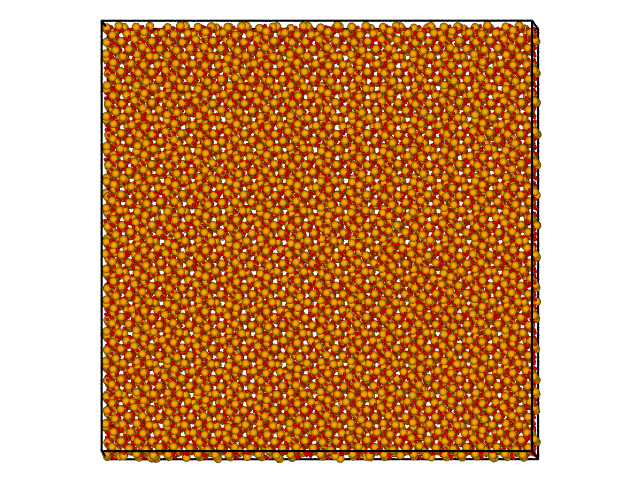
\includegraphics[width=0.22\textwidth]{graphics/initial_atoms.png}
    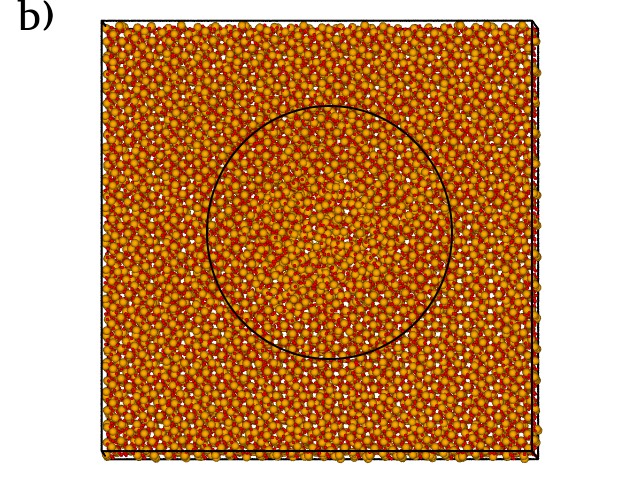
\includegraphics[width=0.22\textwidth]{graphics/spike_atoms.png}
    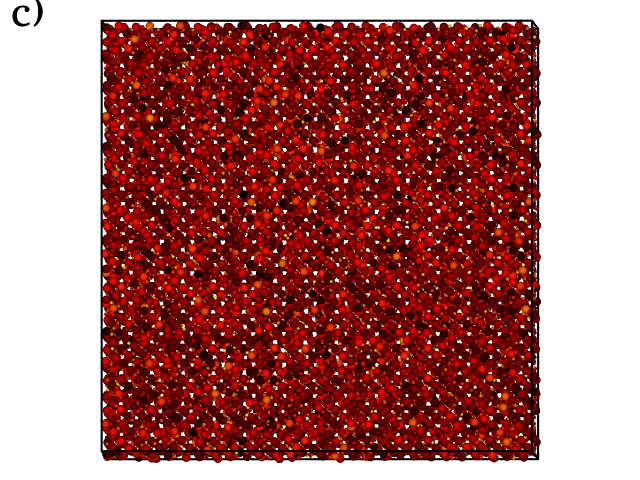
\includegraphics[width=0.22\textwidth]{graphics/initial.png}
    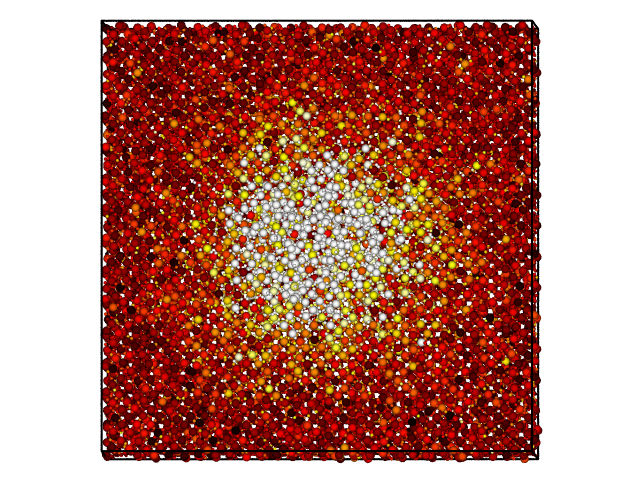
\includegraphics[width=0.22\textwidth]{graphics/spike.png}
  
  \caption{ \textbf{Silica Before and After Swift Heavy Ion Bombardment} View down the SHI pathway. Before: (a) and (c) After: (b) and (d). In (a) and (b), color by type with silicon atoms as \color{Dandelion} yellow \color{black} and the oxygen atoms as \color{BrickRed} red \color{black}. In (c) and (d), atoms are colored by velocity (increasing from \color{BrickRed} red \color{black} $\to$ \color{Dandelion} yellow \color{black} $\to$ \color{black} white). Black circles in (b) and (d) highlight amorphized region.}\label{shi_track}
  \end{center}
\end{wrapfigure}

Previous studies have looked at the fine structure of SHI tracks in amorphous silica using non-equilibrium MD modeling and simulation techniques \cite{Kluth2008, Kluth2011}. The non-equilibrium MD calculations were carried out using the simple approach of instantaneous heating of the atoms in the simulation cell to produce the SHI track path. This method has been motivated by the fact that most of the energy transfer from the electronic system to the atomic degrees of freedom occurs on the femtosecond timescale \cite{ Krasheninnikov2010}.  The timescale of ionic displacements is much greater, implying the transfer is immediate. These non-equilibrium MD simulations of an ion bombardment event, or cascade simulations, are sensitive to the system size where one does not want the radial dispersion of kinetic energy to reach the periodic boundary (in fact, one hopes the cascade dampens well before this boundary). This indicates a large system size is necessary. Also, multiple cascade simulations must be realized to produce an ensemble of events so averaging can be carried out for statistically meaningful results.

We intend to carry out similar simulations of comparable and larger size (~500k to 1M atom simulations) to those of previous studies that can be used to elucidate the structural changes observed in neutron scattering experiments of the average and local structure of different polymorphs of silica from a range of ion bombardment energies (up to GeV energies). Atomistic configurations from these MD trajectories can then be used to carry out RMC modeling to optimize the structure against neutron total scattering data, collected at the Nanoscale Ordered Materials Diffractometer (NOMAD) at the SNS. The results of this study can help understand the fundamental degradation of silica materials undergoing radiation damage \cite{Duffy2007, Rutherford2007} and also to future work to manipulate nanoclusters within solid silica materials using ion bombardment\cite{Ridgway2011}. 

Using the instantaneous kinetic energy deposition technique to simulate the SHI bombardment event is good for a first order approximation. An extension of this project would be to incorporate recent, more realistic modeling \cite{Duffy2007, Rutherford2007, Phillips2010, Leino2015, Khara2016} of the electronic heat conduction to the atomic degrees of freedom. In these models, the solution of the electronic heat conduction is embedded into the MD simulations via including an electronic continuum used to solve the heat equation for modeling the energy transport between the atomic and electronic subsystems. The two-temperature model formalism of including the electron-phonon coupling has been previously used in modeling and simulating SHI bombardment of alpha-quartz, laser ablation, and shock simulations \cite{Phillips2010}. For the ICE-MAN project, this extension would allow us to bridge a quantum-to-classical multiscale-modeling barrier. An important input parameter into the two-temperature model is the electronic specific heat. Recently, it has been shown that the electronic temperature dependence of the electronic specific heat can have an effect on the morphology of the SHI track that is formed \cite{Leino2015, Khara2016}.  To produce this relation, one calculates the difference in internal energy with change in the electronic temperature using finite-temperature density functional theory (DFT). Previous work of others have used the popular Quantum ESPRESSO \cite{Giannozzi2009, QEwebsite} and the VASP \cite{Kresse1996, Kresse1996a, VASPwebsite} softwares to carry out these calculations. Thus, we hope to use this project as a proof-of-concept workflow for ICE-MAN to: begin with quantum calculations, use outputs of these calculations as inputs into non-equilibrium MD simulations, and then use the atomic configurations of outputs from these simulations as inputs into RMC modeling to optimize the atomic structures against neutron scattering data. The SHI workflow will not be a single-use case. Neutron scattering experiments have already been discussed for 2017 to look at other irradiated nuclear waste glass materials before and after irradiation.
